\documentclass[AcMaster]{BJTU-thesis}

%%%%%%%%%%%%%%%%%%%引入一些包%%%%%%%%%%%%%%%%%%%%%55
\usepackage[ruled,linesnumbered]{algorithm2e}
\usepackage{bicaption}
\usepackage{emptypage}
\usepackage{pdfpages}
% \usepackage{enumerate}
%\usepackage{subfig}
%\usepackage{subfig}
%   \setromanfont{Times New Roman}
 \usepackage{fontspec}
 \newfontfamily\myfont{times.ttf}
% \setromanfont[
% BoldFont=timesbd.ttf,
% ItalicFont=timesi.ttf,
% BoldItalicFont=timesbi.ttf,
% ]{times.ttf}
% 
% \setmainfont{Times New Roman}
\renewcommand\labelenumi{(\theenumi)}
\renewcommand{\algorithmcfname}{算法}

\DeclareMathOperator*{\argmin}{argmin}
\DeclareMathOperator*{\argmax}{argmax}

\captionsetup[figure][bi-first]{name=图}
\captionsetup[figure][bi-second]{name=Figure}

\captionsetup[table][bi-first]{name=表}
\captionsetup[table][bi-second]{name=Table}

%%%%%%%%%%%%%%定义一些东西%%%%%%%%%%%%%%%%%%%%%

%\newcommand{\E}{\mathbb{E}}


%\theoremstyle{plain} \theorembodyfont{\kai\rmfamily}
%\theoremheaderfont{\hei\rmfamily}\theoremseparator{.  }

\newtheorem{theorem}{定理}[section]
%\newtheorem{Theorem}{定理}[section]
\newtheorem{lemma}[theorem]{引理}
\newtheorem{corollary}[theorem]{推论}
%\newtheorem{corollary}[theorem]{推论}
\newtheorem{assumption}{假设}[chapter]
%		\newtheorem{Corollary}[Theorem]{推论}
%\newtheorem{Remark}[Theorem]{注}
\newtheorem{example}[theorem]{例}
\newtheorem{definition}[theorem]{定义}
%\newtheorem{Construction}[Theorem]{构造}
%		\def\binom#1#2{{#1\choose#2}}

\newcommand{\E}{\mathbb{E}}
\newcommand{\huaf}{\mathcal{F}}
\newcommand{\huao}{\mathcal{O}}
\newcommand\numberthis{\addtocounter{equation}{1}\tag{\theequation}}
\newcommand{\mne}{ \mathbf{MNE}}
\newcommand{\mnbe}{ \mathbf{MNBE}}

\SetKwInput{KwIn}{输入}
\SetKwInput{KwOut}{输出}


\graphicspath{{./figure/}}

%%%%%%%%%%%%%%%填写封面信息%%%%%%%%%%%%%%%%%%%%
\author{张三}
\studentNumber{11111111}
\advisor{李四老师 }
 
\advisorTitle{教授}
 
\degreeType{理学}
\major{概率论与数理统计}
\researchArea{xxx}
\title{论文题目}
\englishtitle{论文英文题目}
%%%%%%%%%%%%%%%%%%%%%%%%%%%%%%%%%%%%%%%%%%%%%%
%\setmainfont{Times New Roman}

%\makeindex
\makeindex[name=class,options=-s mystyle,title=分类索引,columns=2]
\makeindex[name=author,options=-s mystyle,title=著者索引,columns=2]
\makeindex[name=keyword,options=-s mystyle,title=关键词索引,columns=2]
\begin{document}
	
\makecover
\makeAuthorization

\includepdf[page=-]{chapters/empty.pdf}
\makeInfo
%\include{chapters/thanks}
	\begin{thanks}
		
[内容为小四号宋体。]放置在摘要页前,对象包括:1)国家科学基金,资助研究工作的奖学金基金,合同单位,资助或支持的企业、组织或个人。2)协助完成研究工作和提供便利条件的组织或个人。3)在研究工作中提出建议和提供帮助的人。4)给予转载和引用权的资料、图片、文献、研究思想和设想的所有者。5)其他应感谢的组织和个人。
		
	\end{thanks}
 




% 
\begin{abstract}

  
 [鼠标左键单击选择该段落,输入替换之。内容为小四号宋体。] 中文摘要应将学位论文的内容要点简短明了地表达出来,硕士学位论文一般为500~1000字,博士学位论文一般为1000~2000字。留学生英文版学位论文不少于3000字中文摘要,留学生英文版博士学位论文不少于5000字中文摘要。字体为宋体小四号。内容应包括工作目的、研究方法、成果和结论。要突出本论文的创新点,语言力求精炼。为了便于文献检索,应在本页下方另起一行注明论文的关键词(3-8个),如有可能,尽量采用《汉语主题词表》等词表提供的规范词。图X幅,表X个,参考文献X篇。

\keywords{[请输入关键词(3-8),以分号分隔。] }



    \end{abstract}
\begin{englishabstract}
  
  Ongoing research aims to address these challenges and promote the development of responsible AI technologies. Ongoing research aims to address these challenges and promote the development of responsible AI technologies. 
  Ongoing research aims to address these challenges and promote the development of responsible AI technologies. 
  
\noindent	
\englishkeywords{english keywords}
\end{englishabstract}




%%%\begin{preface}
[鼠标左键单击选择该段落,输入替换之。内容为小四号宋体。] 学位论文的序或前言,一般是作者或他人对本篇论文基本特征的简介,如说明研究工作缘起、背景、主旨、目的、意义、编写体例,以及资助、支持、协作经过等;也可以评述和对相关问题发表意见。这些内容也可以在正文引言中说明。 
\end{preface}
\tableofcontents


\includepdf[page=-]{chapters/empty.pdf} %%%%%注意,这里是在目录后加一个空白页,如果不需要空白页,请注释掉这一行

%%%%%注意,这里如果不需要空白页,请注释掉这一行↑
%%%%%注意,这里如果不需要空白页,请注释掉这一行↑\\
%%%%%注意,这里如果不需要空白页,请注释掉这一行↑\\
%%%%%注意,这里如果不需要空白页,请注释掉这一行↑\\
%%%%%注意,这里如果不需要空白页,请注释掉这一行↑\\





\newpage\pagenumbering{arabic}
%% 引言
		
		\chapter{引言}
		
	 
		
		
		\section{研究背景}
		
		
 
		\begin{figure}[h]
			\centering 
			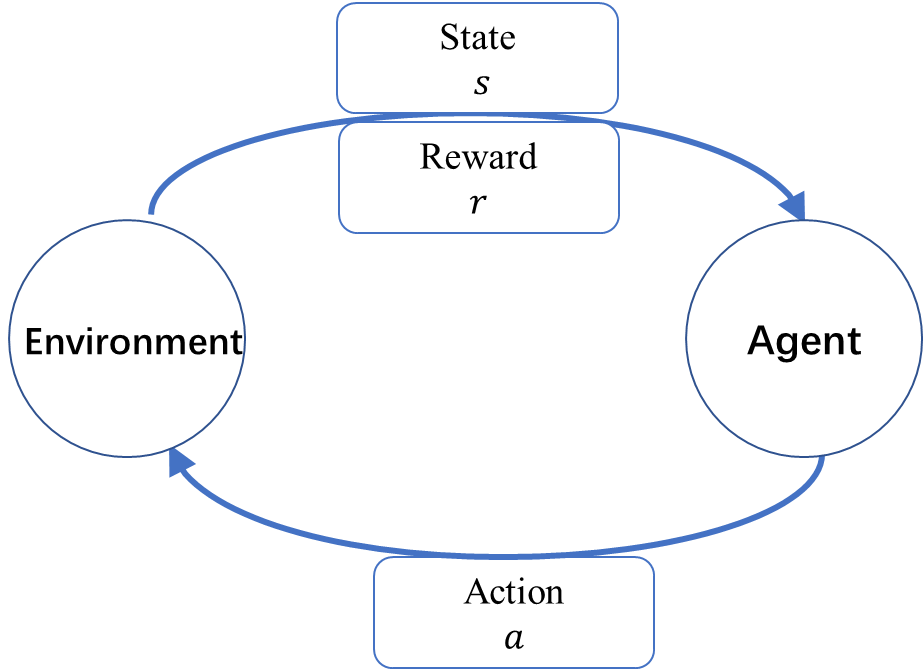
\includegraphics[width=3in,height=2in]{rlp}
	   % 	\caption{  PSI transformation for RNN}
			\bicaption{  序列决策问题示例}{Illustration for sequential decision making problem}
			\label{fig:chap1 rlp}
		\end{figure}

  
  
  
		
		
		\section{本文的结构安排}
		文本的结构安排如下:
 


	 \section{参考文献示例}
参考文献bib文件放在reference文件夹中,在主文件demo中引用了bib文件,在所有chap中都可以直接cite。比如\cite{silver2016mastering}

\section{算法框示例}

\begin{algorithm}[h]
	\caption{ 优化算法}
	\label{gtdmc:alg:minmax}			
	\KwIn{ 迭代次数$ T$,   待学习参数初始值$x_1$ 、 $y_1$ , 学习率 $\alpha$ }
	\For{$ t = 1, \dots, T $}{
		更新参数:  
		
		$ y_{t+1} = \mathcal{P}_{\mathcal{X}_y}\left(y_t + \alpha_t(\hat{b}_t - \hat{A}_t x_t -\hat{M}_ty_t)\right)  $
		
		$ x_{t+1} = \mathcal{P}_{\mathcal{X}_x}\left(x_t + \alpha_t\hat{A}_t^\top y_t\right) $
	}
	
	
	\KwOut{ 		$ \quad 	 \tilde{x}_T = \frac{\sum_{t=1}^{T}\alpha_t x_t}{\sum_{t=1}^{T}\alpha_t}  \qquad \tilde{y}_T = \frac{\sum_{t=1}^{T}\alpha_t y_t}{\sum_{t=1}^{T}\alpha_t} $	 }				
	
	
\end{algorithm}	 

\section{图片示例}



\begin{figure}[h]
	\centering
	\subfloat[a]{
		\label{figa}
		
\includegraphics[width=1.8in,height=1.5in]{a.png}}
	\subfloat[b]{
		\label{figc}
		
\includegraphics[width=1.8in,height=1.5in]{a.png}} 
	\subfloat[c ]{
		\label{fige}
		
\includegraphics[width=1.8in,height=1.5in]{a.png}}	
	
	
	\subfloat[d ]{
		\label{figb}
		
\includegraphics[width=1.8in,height=1.5in]{a.png}}
	\label{Fig1}	
	\subfloat[e ]{
		\label{figd}
		
\includegraphics[width=1.8in,height=1.5in]{a.png}}	
	\subfloat[f ]{
		\label{figf}
		
\includegraphics[width=1.8in,height=1.5in]{a.png}}		
	\bicaption{你好,世界}{Hello world } 
	\label{fig1}
\end{figure}	

%%%% \include{chapters/background}
 
\chapter{总结与展望}

 总结与展望
 
 
 
 
 暖洋洋的太阳照耀着都市的大街。公园里和道路旁已经处处绿意朦胧。风中飘着一团团
 雪白的杨絮。街心花园的第一批鲜花,也在不知不觉中竞相开放了。古城的春天稍显即逝,
 人们立刻就有一种身临初夏的感觉。
 街头的行人稠密起来。人们纷纷走出户外,尽情享受阳光和暖风的抚爱。那些时髦的姑
 娘已经过早地脱掉了外套,穿起单薄的、色彩鲜艳的毛衣线衣。到处传来春游的孩子们的歌
 声。城市一改冬日的灰暗,重新显出了它那多彩的风貌。
 孙少平的伤已经完全好了。雷汉义区长代表矿上来为他办出院手续。他准备过几天就返
 回大牙湾。
 
 这期间,妹妹兰香和她的男朋友仍然一直给他做工作,让他调到省城来。他到现在还没
 有完全拒绝他们的好意。尽管他对自己未来的生活心中有数,但不好当面向他们进一步解释
 他的想法。他们应该意识到,他和他们的处境不尽相同。不同生活处境的人应该寻找各自的
 归宿。大城市对妹妹和仲平也许是合适的,但他在这里未必能寻找到自己的幸福。他想等以
 后适当的时间用另一种方式向他们说明自己的观点和态度。
 其实,这期间最使他伤神的倒不是兰香和仲平一再劝他来省城工作。他苦恼的是金秀对
 他表示的热烈感情。自从她把那封恋爱信送到他手中,他就一直苦苦思索自己该怎么办?
 秀可爱吗?非常可爱!她是那样的热情,漂亮;情感炽热而丰富,一个瞬间给予男人的
 东西都要比冷血女人一生给予的还要多。她使他想起了死去的晓霞。她也是大学生,有文
 化,有知识,有很好的专业。她无疑会是一个令男人骄傲的妻子。双方感情交流也没什么障
 碍,他们从小一块长大,一直以兄妹相待;这种关系如果汇入夫妻生活,那将是十分美好
 的。
 
 秀要成为他的妻子?他要成为秀的丈夫?他一时又难以转过这个弯。他一直把秀当小妹
 妹看待;在他眼里,她永远是个小孩子,怎么能和她一块过夫妻生活呢?想到这一点,他就
 感到别扭。
 
 当然,最重要的是,他和秀的差异太大了。他是一个在井下干活的煤矿工人,而金秀是
 大学生,他怎么能和她结婚?秀在信上说她毕业后准备去他所在的矿医院当医生。他相信她
 能真诚地做到这一点。但他能忍心让她这样做吗?据兰香一再给他说,按金秀的学习情况,
 她完全可以考上研究生。他为什么要耽搁她的前程?如果因为他的关系,让秀来大牙湾煤
 矿,实际上等于把她毁了。他现在才记起,他曾给金波也说过这个意思。
 所有这一切考虑,不是说没勇气和一个女大学生一块生活。当年田晓霞也是大学生、记
 者。但秀和晓霞又不一样。晓霞在总体素质上是另一种类型的女性。虽然他和秀一块长大,
 但秀决不会象晓霞那样更深刻地理解他。他和秀之间总有一种隔代之感。
 怎么办?这比兰香和仲平要他来大城市工作更难以回答。他知道秀在热切地等待他的回
 话。给他交了那封信后,她尽管和往常一样细心而入微地照料他,但他们之间已明显地产生
 了一种极不好意思的成份……生活是这样令人感慨不已!
 孙少平不由想起十年前他的初恋。他想起了他爱上的第一个女人郝红梅。富有戏剧性的
 是,十年前的那场感情纠葛发生在他和顾养民之间;没想到十年后,他又和顾养民纠缠在一
 起。不同的是,十年前,郝红梅离他而去爱顾养民;而今天,金秀却要离开顾养民而爱他
 了!
 
 生活似乎走了一个令人难以置信的圆。
 
 但生活又不会以圆的形式结束。生活会一直走向前去!瞧,十年过去了,所有人的生活
 都发生了多么大的变化。就拿他们几个说吧,养民已经到上海去读研究生;而前不久他震惊
 地获悉,郝红梅带着前夫留下的孩子,竟然和他同村的另一个同学田润生结了婚,现在就生
 活在双水村。而他,当了一名干粗活的煤矿工人,现在受了伤,住了院,却被养民爱着的金
 秀爱上了……直到现在,他也不知如何与金秀谈这件事。他能感觉来,秀对他的爱是多么强
 烈!他不能用简单的三言两语来拒绝她,这样会伤害孩子……是的,孩子。他现在还认为秀
 是个孩子!但是,他又不能简单地响应她爱情的呼唤。如果是那样,那伤害的不仅是秀,还
 有他自己的心灵。
 
 孙少平左思右想,不知他该怎么办。
 
 想不出个妥当的结果,他就不能轻易对她表示什么。好在他很快就要离开省城;等离开
 时,说不定他能对这件事做出结论性的决定……
 区长雷汉义帮他结完手续后,他就算和医院告别了。他让区长先回去,他自己还想在省
 城逗留几天;他知道,他还有些“事”需要处理。
 
 雷汉义临走时,才迟疑着从衣袋里摸出两份矿上的文件给了他。
 孙少平一看,这两份文件都是有关他自己的。一份是通报表彰他舍己救人的献身精神;
 另一份是批评他作为班长,元旦那天让喝醉酒的工人下井,违反了规章制度,决定给他记大
 过一次。
 
 孙少平把两份文件揉成一团,塞进了自己的衣袋里。雷汉义安慰他说:“不管是表彰,
 还是处分,都是些球!回去只管掏咱的炭!”
 但孙少平的心情却是沉重的。这是一种永远不能互相抵消的存在,就象他五官正常的脸
 上那道丑陋的疤痕。他倒并不特别看重这两份让他哭笑不得的文件,而是由此伤感地想到,
 这正好说明了他那负重前行的生存处境。
 仲平竭力要求出院后的少平到他家去。但他谢绝了。兰香理解二哥的心情,也没有再坚
 持。少平随即住进了一家个体户开办的小旅店。
 他住进旅店后的第一件事,就是给惠英和明明写了一封信,告诉他什么时候回大牙湾煤
 矿。
 
 几天之后,在少平即将离开省城的时刻,金秀和兰香相跟着来旅店找他,想陪他出去到
 街上转转。但少平推诿着不想去。最少在眼下,他不愿带着脸上的疤痕,和任何女性相跟着
 逛大街,他无法忍受陌生人用异样的目光看他和身边两个漂亮的妹妹。说实话,对脸上的那
 道疤痕,尽管他显得不在乎,但内心却为此而万般痛苦,爱美之心人人有,更何况,他正当
 青春年华!至于他的脸倒究被毁到了何种程度,直到现在他都没有勇气去照镜子。
 金秀见他执意不到街上去转,就提议他们三个人一块到她的宿舍去坐坐;她说她们宿舍
 实习的同学都没回来,就她一个人。医学院离这儿很近,少平也就同意了。金秀本来不想让
 兰香去,但她有口难言。
 
 三个人到医学院金秀的宿舍后,秀特意让少平坐到她床上休息。她让少平先一个人待一
 会,自己随即又拉了兰香,到外面去采买吃的——她想好好款待一下少平哥。
 兰香和金秀走后,少平一个人没事,就在秀的枕头边拿了几本医学杂志看。他在无意间
 发现秀床铺那头的墙上挂一面圆镜子。他犹豫了一下,过去摘下那面镜子。当镜子就要举到
 面前的时候,他闭住了眼睛。
 
 他闭着眼,举着镜子,脚步艰难地挪到了靠近房门的空地上。他久久地立着,拿镜子的
 那条胳膊抖得象筛糠一般。在这一刻里,孙少平不再是血性男儿,完全成了一个胆怯的懦
 夫!
 
 我看到的将会是怎样的一个我?他在心里问自己。你啊!为什么不敢正视自己的不幸
 呢?你不愿看见它,难道它就不存在吗?你连看见它的勇气都鼓不起来,你又怎样带着它回
 到人们中间去生活?可笑。你这可笑的驼鸟政策!
 他睁开了眼睛。呀!他看见,那道可怕的伤疤从额头的发楞起斜劈过右眼角,一直拉过
 颧骨直至脸颊,活象调皮孩子在公厕墙上写了一句骂人话后所划下的惊叹号!
 他猛地把那面镜子摔在水泥地板上;一声爆响,镜子的碎片四处飞溅。接着,他一下伏
 在金秀的床铺上,埋住脸痛哭起来……
 他听见了敲门声——是秀和兰香回来了。
 他爬起来,用秀的毛巾揩去了脸上的泪痕。接着,匆忙地拿起扫帚,把满地的碎镜片扫
 到门后。在手捉住门锁柄的时候,他停留片刻,以便自己镇静下来——尽管他知道这是徒劳
 的。
 在门打开的一刹那间,他看见两个妹妹都怀里抱着一堆吃的东西,脸色苍白地愣住看
 他。她们显然感到这屋里曾发生了什么事。其实,他自己的神态就说明了这一点。
 不过,她们很快说笑着走过来了。以后,她们一直装着没有看见门背后的那一堆碎镜
 片。
 两个女孩子象演戏一样,大声说笑着,甚至有点咋咋唬唬,在桌子上铺开了块干净的白
 布,然后把那些罐头、啤酒、果子露、牛肉、面包等等吃的东西都摆好,让他坐到“上席”
 上,并且开玩笑称他“革命老前辈”……吃过东西后,少平没让她们送他,自己一个人来到
 大街上。
 
 啊,最为严重的时刻也许已经过去了!
 现在,他行走在这人流如潮的大街上,不管有多少含义复杂的目光在他脸上扫射,他也
 坦然如常。不知为什么,他甚至感到自己的情绪渐渐亢奋起来。
 他在个体户的小摊上买了一副黑镜,随即就戴起来——部份地遮掩了脸上那道疤痕。接
 着,他又到商店买了一件铁灰色风雨衣穿在身上。这打扮加上脸上那道疤,奇特地使他具有
 了另一种男子汉的魅力——这正是他想象中自己的“新”形象。在下午剩下的最后一点时光
 里,他还到新华书店买了几本书。其中他最喜欢的一本书是《一些原材料对人类未来的影
 响》。
 
 当天晚上,他静静地坐在小旅店的房间里,分别给妹妹、仲平和金秀写了两封信。在给
 兰香和仲平的信中,他向他们“阐述”了他为什么现在不想来大城市工作的想法。他说他也
 许一辈子可能和煤炭打交道。在给金秀的一封很长的信中,他主要向她表明为什么他不能和
 她结合的理由。他祝愿亲爱的金秀妹妹和顾养民或别的一个男人幸福地生活……第二天,孙
 少平提着自己的东西,在火车站发出了那两封信,就一个人悄然离开了省城。
 中午时分,他回到了久别的大牙湾煤矿。
 
 他在矿部前下了车,抬头望了望高耸的选煤楼、雄传的矸石山和黑油油的煤堆,眼里忍
 不住涌满了泪水。温暖的季风吹过了绿黄相间的山野;蓝天上,是太阳永恒的微笑。
 他依稀听见一支用口哨吹出的充满活力的歌在耳边回响。这是赞美青春和生命的歌。
 他上了二级平台,沿着铁路线急速地向东走去。他远远地看见,头上包着红纱巾的惠
 英,胸前飘着红领巾的明明,以及脖项里响着铜铃铛的小狗,正向他飞奔而来……准备:1
 982年—1985年第一稿:1987年秋天—冬天第二稿:1988年春天—夏天[全
 书完]
 
 这五卷文集可以说是我四十岁之前文学活动的一个基本总结。其间包含着青春的激情,
 痛苦和失误,包含着劳动的汗水、人生的辛酸和对这个冷暖世界的复杂体验。更重要的是,
 它也包含了我对生活从未淡薄的挚爱与深情。至此,我也就可以对我的青年时代投去最后一
 瞥,从而和它永远告别了。
 这五卷文集的出版,得益于陕西人民出版社和本书编选者陈泽顺、刑良俊同志,没有他
 们的热情帮助,这件事是不可能做成的。
 我庆幸降生于这个伟大而值得自豪的国度。它深厚的历史文化,辽阔的疆土和占地球的
 五分之一的人口,使得其间任何人的劳动都能得到广大的支持,同时也发生广大的影响。无
 论我们曾经历了多少痛苦和磨难,且还将要面对多少严峻考验:也不论我们处于何种位置何
 种境地,我们都会为能服务于伟大的祖国和如此众多的同胞而心甘情愿地献出自己毕生的精
 力和才智。
 我感谢我所生活的这个充满戏剧性的时代,也感谢与我生活在这同一时代的人们。所有
 这一切历史构成,都给我提供了一种人生的契机,使我意外地有可能如愿从事自己钟爱的文
 学事业,将自己的心灵和人世间无数的心灵沟通。正是千千万万我的同时代读者一次又一次
 促我投入也许并不是我完全能胜任的艰巨工作。现在,我总算能将自己的一些微不足道的收
 获献给我的读者朋友。
 那么,对于一个原本一无所有的农民的儿子,还有什么不满足呢?
 是的,不满足。我应该把一切进行得比现在更好。历史,社会环境,尤其是个人的素
 养,都在局限人——不仅局限艺术作品中的人,首先局限它的创造者。所有人的生命历程在
 人类历史的长河中都是一个小小的段落,因此,每一代人都有自己的命中注定的遗撼。遗
 撼,深深的遗撼。
 唯一能自慰的是,我们曾真诚而充满激情地在这个世界上生活过,竭尽全力地劳动过,
 并不计代价地将自己的血汗献给了不死的人类之树。
 在我们的世界发生激烈演变的大潮中。人类社会将以全然不同于以往的面貌进入另一世
 纪。我们生而逢时,不仅可以目睹一幕紧接一幕的大剧,也将不可避免地要在其间扮演某种
 属于自己的角色。现实生活中的任何人都不可能逃避自己历史性的责任。无疑,在未来的年
 月里,生活和艺术都会向作家提出更为繁难而严厉的要求。如果沉醉满足于自己以往的历史
 就无异于生命大限的终临,人生旅程时刻处于“零公里”处。那么,要旨仍然应该是首先战
 胜自己,并将精神提升到不断发展着的生活所要求的那种高度,才有可能使自己重新走出洼
 地,亦步亦趋跟着生活进入新的境界。不管实际结果如何,这个起码的觉悟应当具备。
 结论一目了然:只能永远把艰辛的劳动看作是生命的必要;即使没有收获的指望,也心
 平气静地继续耕种。1992年春天于西安
	
\bibliography{reference/ref}
%% 附录
%\appendix
% \chapter[附录标题]{}
%	\addcontentsline{toc}{section}{附录\thechapter\hspace*{1em}附录标题}
\markboth{附录\thechapter}{}
\begin{center}
	\zihao{3}\bfseries 附录标题
\end{center}

[内容为五号宋体。] 附录是作为论文主体的补充项目,并不是必须的。
论文的附录依序用大写正体英文字母A、B、C……编序号,如:附录A。


%正文中加入index:
%This is my key\index{key}.
%This is my second palace\index[class]{palace} that has a key.



\index{classfication!plus}	
%%% 索引
%\chapter*{索引}
%\pagestyle{fancy}
%\addcontentsline{toc}{chapter}{索引}
%678
%\printindex[class]
%\addcontentsline{toc}{section}{分类索引}
%456
%\printindex[author]
%\addcontentsline{toc}{section}{著者索引}
%345
%\printindex[keyword]
%\addcontentsline{toc}{section}{关键词索引}
%123



	\chapter*{作者简历及攻读硕士/博士学位期间取得的研究成果}
	\markboth{作者简历及攻读硕士/博士学位期间取得的研究成果}{}
\addcontentsline{toc}{chapter}{作者简历及攻读硕士/博士学位期间取得的研究成果}
%	[内容采用五号宋体]  包括教育经历、工作经历、攻读学位期间发表的论文和完成的工作等。行距16磅,段前后各为0磅。
	
一、作者简历

	\textbf{基本情况:}
	
 
	\textbf{教育经历:}
	
 
	
	\textbf{研究兴趣:}
	
	 
	
	
二、发表论文
	\setlength\leftmargini{3.5em}
	\renewcommand\labelenumi{[\theenumi]}
	\begin{enumerate}
	\item Silver D, Schrittwieser J, Simonyan K, et al. Mastering the game of go without human knowledge[J]. Nature, 2017, 550(7676): 354-359.

	\end{enumerate}

	三、参与科研项目
	\begin{enumerate}
		\item e
		\item yi
		\item san
	\end{enumerate}

	四、专利
	\begin{enumerate}
		\item e
		\item yi
		\item san
	\end{enumerate}
%%% 独创性声明	
\chapter*{独创性声明}
\markboth{独创性声明}{}
\addcontentsline{toc}{chapter}{独创性声明}
本人声明所呈交的学位论文是本人在导师指导下进行的研究工作和取得的研究成果,除了文中特别加以标注和致谢之处外,论文中不包含其他人已经发表或撰写过的研究成果,也不包含为获得北京交通大学或其他教育机构的学位或证书而使用过的材料。与我一同工作的同志对本研究所做的任何贡献均已在论文中作了明确的说明并表示了谢意。

\vspace*{3em}
学位论文作者签名:\hfill 签字日期:\hspace*{4em}年\hspace*{2em}月\hspace*{2em}日
%% 学位论文数据集
%\chapter*{学位论文数据集}
\markboth{学位论文数据集}{}
\addcontentsline{toc}{chapter}{学位论文数据}
% Table generated by Excel2LaTeX from sheet 'Sheet1'
\begin{table}[htbp]
	\centering
	\caption{数据集页}
	\begin{tabular}{|p{6.94em}rrrr|}
		\hline
		\multicolumn{1}{|p{6.94em}|}{关键词*} & \multicolumn{1}{p{6.065em}|}{密级*} & \multicolumn{1}{p{6.625em}|}{中图分类号} & \multicolumn{1}{p{7em}|}{UDC} & \multicolumn{1}{p{6.69em}|}{论文资助} \\
		\hline
		\multicolumn{1}{|r|}{} & \multicolumn{1}{r|}{} & \multicolumn{1}{r|}{} & \multicolumn{1}{r|}{} &  \\
		\hline
		\multicolumn{2}{|p{13.005em}|}{学位授予单位名称*} & \multicolumn{1}{p{6.625em}|}{学位授予单位代码*} & \multicolumn{1}{p{7em}|}{学位类别*} & \multicolumn{1}{p{6.69em}|}{学位级别*} \\
		\hline
		\multicolumn{2}{|p{13.005em}|}{北京交通大学} & \multicolumn{1}{r|}{10004} & \multicolumn{1}{r|}{} &  \\
		\hline
		\multicolumn{2}{|p{13.005em}|}{论文题名*} & \multicolumn{2}{p{13.625em}|}{并列题名} & \multicolumn{1}{p{6.69em}|}{论文语种*} \\
		\hline
		\multicolumn{2}{|r|}{} & \multicolumn{2}{r|}{} &  \\
		\hline
		\multicolumn{1}{|p{6.94em}|}{作者姓名*} & \multicolumn{2}{r|}{} & \multicolumn{1}{p{7em}|}{学号*} &  \\
		\hline
		\multicolumn{2}{|p{13.005em}|}{培养单位名称*} & \multicolumn{1}{p{6.625em}|}{培养单位代码*} & \multicolumn{1}{p{7em}|}{培养单位地址} & \multicolumn{1}{p{6.69em}|}{邮编} \\
		\hline
		\multicolumn{2}{|p{13.005em}|}{北京交通大学} & \multicolumn{1}{r|}{10004} & \multicolumn{1}{p{7em}|}{北京市海淀区西直门外上园村3号} & 100044 \\
		\hline
		\multicolumn{2}{|p{13.005em}|}{学科专业*} & \multicolumn{1}{p{6.625em}|}{研究方向*} & \multicolumn{1}{p{7em}|}{学制*} & \multicolumn{1}{p{6.69em}|}{学位授予年*} \\
		\hline
		\multicolumn{2}{|r|}{} & \multicolumn{1}{r|}{} & \multicolumn{1}{r|}{} &  \\
		\hline
		\multicolumn{1}{|p{6.94em}|}{论文提交日期*} & \multicolumn{4}{r|}{} \\
		\hline
		\multicolumn{1}{|p{6.94em}|}{导师姓名*} & \multicolumn{2}{r|}{} & \multicolumn{1}{p{7em}|}{职称*} &  \\
		\hline
		\multicolumn{1}{|p{6.94em}|}{评阅人} & \multicolumn{2}{p{12.69em}|}{答辩委员会主席*} & \multicolumn{2}{p{13.69em}|}{答辩委员会成员} \\
		\hline
		\multicolumn{1}{|r|}{\multirow{2}[2]{*}{}} & \multicolumn{2}{r|}{\multirow{2}[2]{*}{}} & \multicolumn{2}{r|}{\multirow{2}[2]{*}{}} \\
		\multicolumn{1}{|r|}{} & \multicolumn{2}{r|}{} & \multicolumn{2}{r|}{} \\
		\hline
		\multicolumn{5}{|p{33.32em}|}{电子版论文提交格式  文本( )  图像( ) 视频( ) 音频( ) 多媒体( ) 其他( )} \\
		\multicolumn{5}{|p{33.32em}|}{推荐格式:application/msword;application/pdf} \\
		\hline
		\multicolumn{2}{|p{13.005em}|}{电子版论文出版(发布)者} & \multicolumn{2}{p{13.625em}|}{电子版论文出版(发布)地} & \multicolumn{1}{p{6.69em}|}{权限声明} \\
		\hline
		\multicolumn{2}{|r|}{} & \multicolumn{2}{r|}{} &  \\
		\hline
		\multicolumn{1}{|p{6.94em}|}{论文总页数*} & \multicolumn{4}{r|}{} \\
		\hline
		\multicolumn{5}{|p{33.32em}|}{共33项,其中带*为必填数据,为21项。} \\
		\hline
	\end{tabular}%
	\label{tab:addlabel}%
\end{table}%

\includepdf[page=-]{chapters/empty.pdf}
 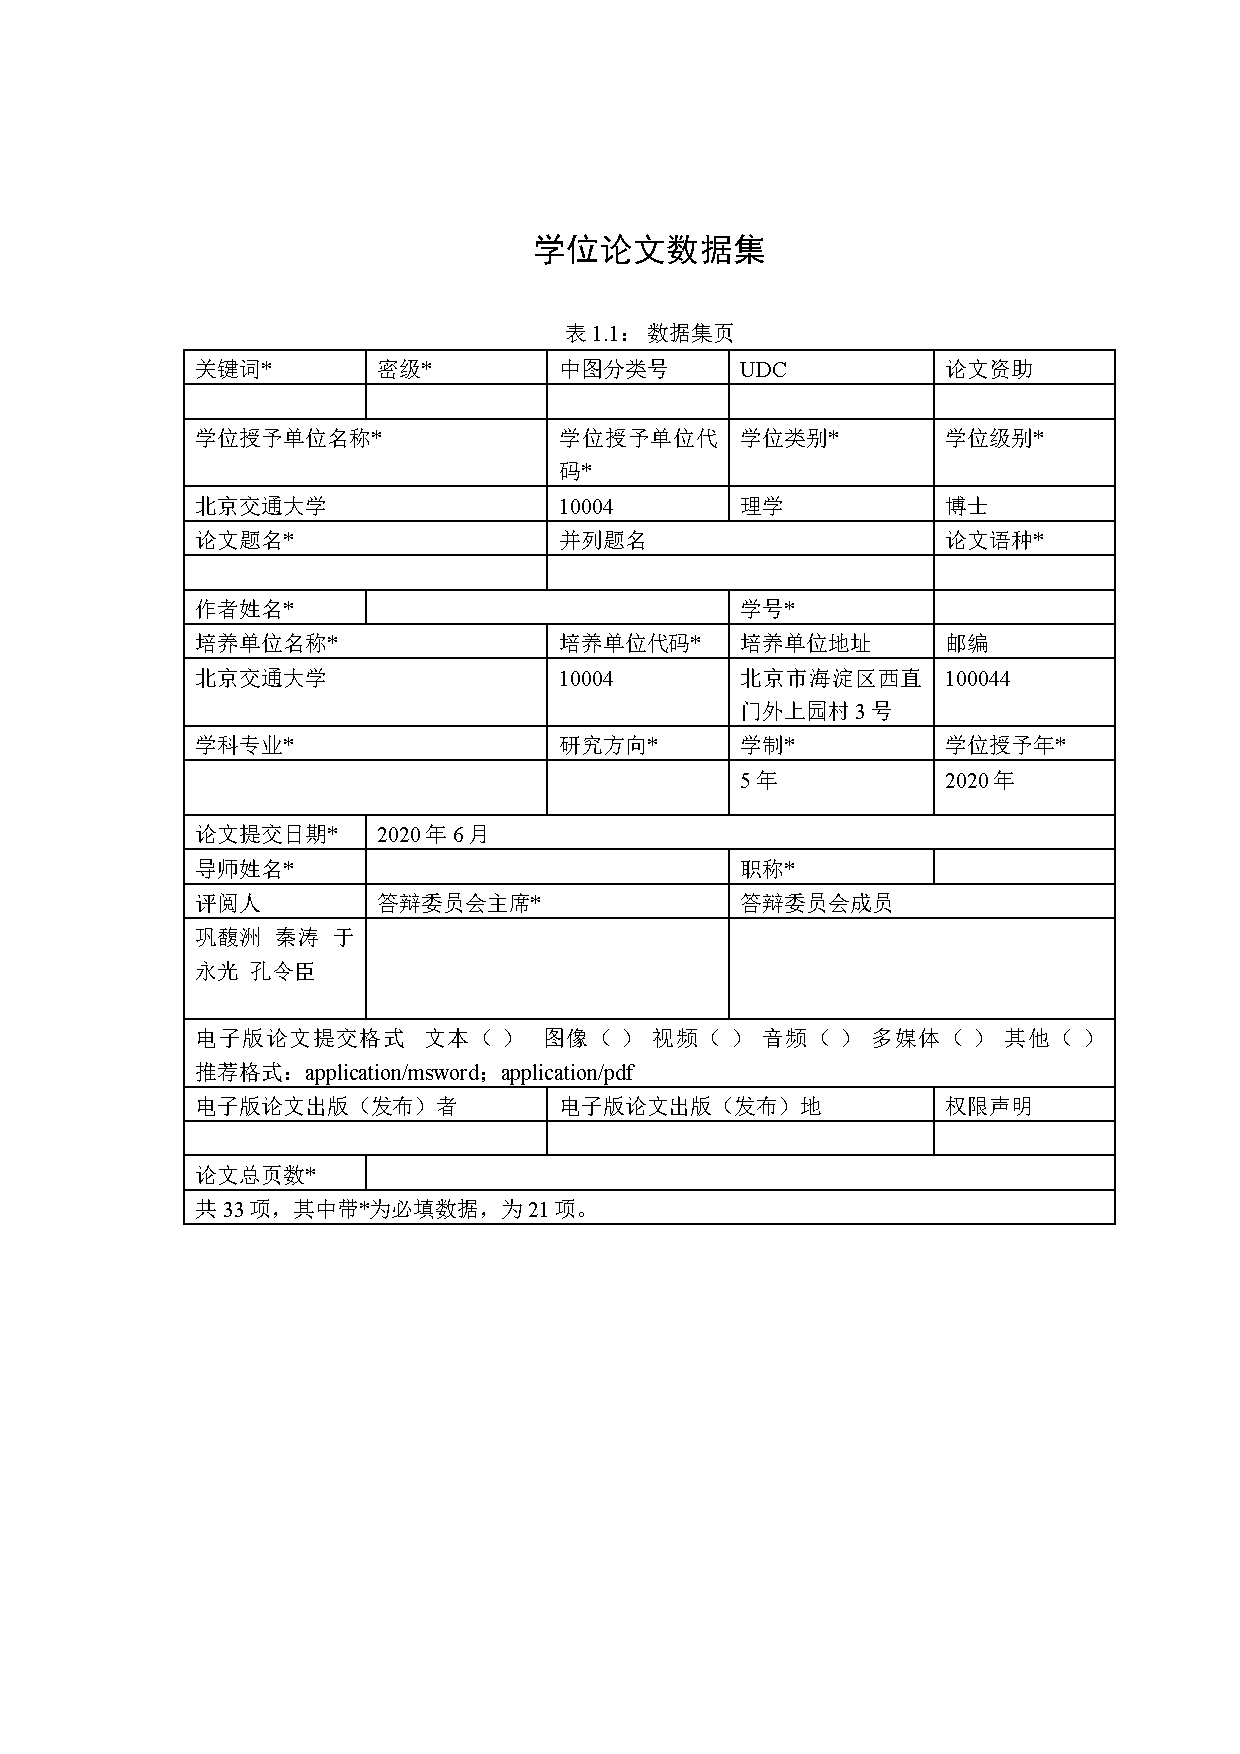
\includepdf[page=-]{chapters/dataset.pdf}

%1232

\end{document}